\documentclass[12pt, twoside]{article}
\documentclass[12pt, twoside]{article}
\usepackage[letterpaper, margin=1in, headsep=0.2in]{geometry}
\setlength{\headheight}{0.6in}
%\usepackage[english]{babel}
\usepackage[utf8]{inputenc}
\usepackage{microtype}
\usepackage{amsmath}
\usepackage{amssymb}
%\usepackage{amsfonts}
\usepackage{siunitx} %units in math. eg 20\milli\meter
\usepackage{yhmath} % for arcs, overparenth command
\usepackage{tikz} %graphics
\usetikzlibrary{quotes, angles}
\usepackage{graphicx} %consider setting \graphicspath{{images/}}
\usepackage{parskip} %no paragraph indent
\usepackage{enumitem}
\usepackage{multicol}
\usepackage{venndiagram}

\usepackage{fancyhdr}
\pagestyle{fancy}
\fancyhf{}
\renewcommand{\headrulewidth}{0pt} % disable the underline of the header
\raggedbottom
\hfuzz=2mm %suppresses overfull box warnings

\usepackage{hyperref}
\usepackage{float}

\fancyhead[LE]{\thepage}
\fancyhead[RO]{\thepage \\ First and last name: \hspace{2.5cm} \,\\ Section: \hspace{2.5cm} \,}
\fancyhead[LO]{BECA / Dr. Huson / Regents Prep: Graphs\\* 21 November 2024}

\begin{document}

\subsubsection*{1.10 Do Now Quiz: Graphing inequalities \& times tables}
\begin{enumerate}
  \item Graph and label the two equations. Mark their intersection as an ordered pair.

  \begin{multicols}{2}
    $y \leq \frac{1}{2}x-2$ \\[0.25cm]
    Write down the slope and $y$-intercept\\ of the first equation.
    \begin{enumerate}
      \item $m=$ \bigskip
      \item $b=$
    \end{enumerate}
    \columnbreak
    $x+y > 4$ \\[0.5cm]
        Write as slope-intercept form, $y=mx+b$.
    \end{multicols}

  \begin{center} %4 quadrant regents grid w T-Chart
  \begin{tikzpicture}[scale=.635]
    \draw [help lines] (-10,-10) grid (10,10);
    \draw [thick, ->] (-10.2,0) -- (10.4,0) node [below right] {$x$};
    \draw [thick, ->] (0,-10.2)--(0,10.4) node [left] {$y$};
  \end{tikzpicture}
  \end{center}

For each equation, lightly shade the side of the line that satisfies the inequality.

\newpage
\subsubsection*{3.OA.7 Fluently multiply and divide within 100}

\item Perform the calculations.
  \begin{multicols}{2}
    \begin{enumerate}[itemsep=1cm]
        \item $2 \times 3 =$
        \item $4 \times 5 =$
        \item $3 \times 2 =$
        \item $5 \times 4 =$
        \item $2 \times 5 =$
        \item $3 \times 4 =$
    \end{enumerate}
  \end{multicols} \vspace{1cm}

  \item Perform the calculations.
  \begin{multicols}{2}
    \begin{enumerate}[itemsep=1cm]
        \item $6 \times 7 =$
        \item $8 \times 9 =$
        \item $7 \times 6 =$
        \item $9 \times 8 =$
        \item $6 \times 6 =$
        \item $7 \times 9 =$
    \end{enumerate}
  \end{multicols} \vspace{1cm}

\item Find each quotient.
  \begin{multicols}{2}
    \begin{enumerate}[itemsep=1cm]
        \item $15 \div 3 =$
        \item $42 \div 7 =$
        \item $27 \div 9 =$
        \item $64 \div 8 =$
        \item $36 \div 6 =$
        \item $35 \div 5 =$
    \end{enumerate}
  \end{multicols}


\end{enumerate}
\end{document}